\documentclass[margin=10pt]{standalone}
\usepackage{tikz}
% \usetikzlibrary{arrows,shapes,positioning}
\usetikzlibrary{arrows.meta}
\usetikzlibrary{calc}

\begin{document}

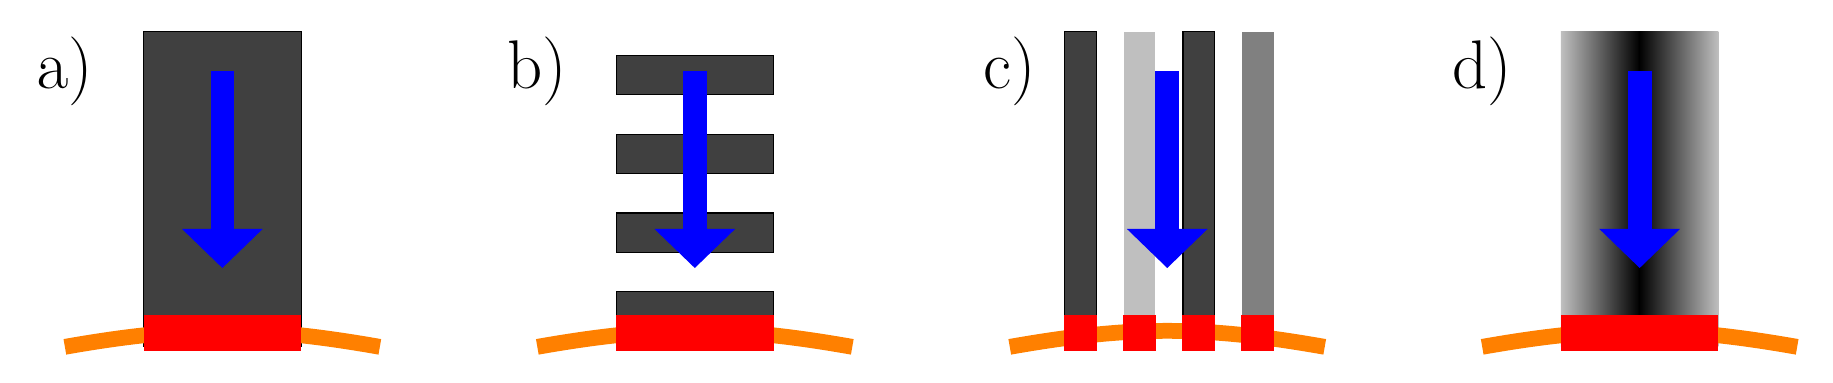
\begin{tikzpicture}
  \begin{scope}
    \draw[fill=darkgray] (1,1) rectangle (3,5);  
    \draw[orange,line width=0.2cm] (0,1) to[out=10,in=170] (4,1);
    \draw[blue, <-, arrows={-Triangle[angle=90:10pt,blue,fill=blue, scale=2.]}, line width=0.3cm] (2,4.5) -- (2,2);
    \fill[red] (1,0.95) rectangle (3,1.4);
  \end{scope}
  
  
  
  
   
    \begin{scope}[shift={(6,0)}, rotate=0]
    \foreach \x in {0,...,3}
      {
        \draw[fill=darkgray] (1,1.2+\x) rectangle (3,1.7+\x);  
      }  
    \draw[orange,line width=0.2cm] (0,1) to[out=10,in=170] (4,1);
    \draw[blue, <-, arrows={-Triangle[angle=90:10pt,blue,fill=blue, scale=2.]}, line width=0.3cm] (2,4.5) -- (2,2);
    \fill[red] (1,0.95) rectangle (3.01,1.4);
  \end{scope}
  
  
  
   \begin{scope}[shift={(12,0)}]
    \draw[orange, line width=0.2cm] (0,1) to[out=10,in=170] (4,1);
    
     \foreach \x in {0,...,1} {
          \draw[fill=darkgray] (0.7+\x*1.5,1) rectangle (1.1+\x*1.5,5); 
     }
     \fill[lightgray] (1.45,1) rectangle (1.85,5);
     \fill[gray] (2.95,1) rectangle (3.35,5); 
    
    \foreach \x in {0,...,3} {
        \fill[red] (0.69+\x*0.75,0.95) rectangle (1.11+\x*0.75,1.4);
    }
        \draw[blue, <-, arrows={-Triangle[angle=90:10pt,blue,fill=blue, scale=2.]}, line width=0.3cm] (2,4.5) -- (2,2);
   \end{scope}

   
   
   
   
  \begin{scope}[shift={(18,0)}]
    \shade[left color=lightgray, right color=black] (1,1) rectangle (2,5); 
    \shade[left color=black, right color=lightgray] (1.99,1) rectangle (3,5); 
%     \draw[fill=darkgray] (1,1) rectangle (3,6);  
    \draw[orange,line width=0.2cm] (0,1) to[out=10,in=170] (4,1);
    \draw[blue, <-, arrows={-Triangle[angle=90:10pt,blue,fill=blue, scale=2.]}, line width=0.3cm] (2,4.5) -- (2,2);
    \fill[red] (1,0.95) rectangle (3,1.4);
  \end{scope}
  
  \node at (0,4.5) {\Huge a)};
  \node at (6,4.5) {\Huge b)};
  \node at (12,4.5) {\Huge c)};
  \node at (18,4.5) {\Huge d)};
  
\end{tikzpicture}

\end{document}
